%%%%%%%%%%%%%%%%%%%%%%%%%%%%%%%%%%%%%%%%%%%%%%%%%%%%%%%%%%%%%%%%%%%%%%%%%%
%                                                                        %
%  The Why platform for program certification                            %
%                                                                        %
%  Copyright (C) 2002-2010                                               %
%                                                                        %
%    Jean-Christophe FILLIATRE, CNRS                                     %
%    Claude MARCHE, INRIA & Univ. Paris-sud 11                           %
%    Yannick MOY, Univ. Paris-sud 11                                     %
%    Romain BARDOU, Univ. Paris-sud 11                                   %
%    Thierry HUBERT, Univ. Paris-sud 11                                  %
%                                                                        %
%  Secondary contributors:                                               %
%                                                                        %
%    Nicolas ROUSSET, Univ. Paris-sud 11 (on Jessie & Krakatoa)          %
%    Ali AYAD, CNRS & CEA Saclay         (floating-point support)        %
%    Sylvie BOLDO, INRIA                 (floating-point support)        %
%    Jean-Francois COUCHOT, INRIA        (sort encodings, hyps pruning)  %
%    Mehdi DOGGUY, Univ. Paris-sud 11    (Why GUI)                       %
%                                                                        %
%  This software is free software; you can redistribute it and/or        %
%  modify it under the terms of the GNU Lesser General Public            %
%  License version 2.1, with the special exception on linking            %
%  described in file LICENSE.                                            %
%                                                                        %
%  This software is distributed in the hope that it will be useful,      %
%  but WITHOUT ANY WARRANTY; without even the implied warranty of        %
%  MERCHANTABILITY or FITNESS FOR A PARTICULAR PURPOSE.                  %
%                                                                        %
%%%%%%%%%%%%%%%%%%%%%%%%%%%%%%%%%%%%%%%%%%%%%%%%%%%%%%%%%%%%%%%%%%%%%%%%%%

\documentclass[a4paper,12pt]{article}

\usepackage[a4paper=true,pdftex,colorlinks=true,urlcolor=blue,pdfstartview=FitH]{hyperref}

\usepackage[T1]{fontenc}

\usepackage{times}
\usepackage{graphicx}
\textwidth=160mm
\oddsidemargin=0mm
\evensidemargin=0mm
\textheight=270mm
\topmargin=-25mm

\renewcommand{\textfraction}{0.01}
\renewcommand{\topfraction}{0.99}
\renewcommand{\bottomfraction}{0.99}

\pagestyle{empty}

\begin{document}
\sloppy

\title{Case study: new features of specification languages}
\author{Claude March\'e}
\date{February 2008}
\maketitle

\thispagestyle{empty}



The following program is not a challenge to prove (although not easy
for automatic provers). It is rather an illustration of new features
we added to our specification languages ACSL (for C programs) and KSL
(Krakatoa Specification Language for Java programs).

The new features are:
\begin{itemize}
\item named behaviors in contracts
\item ghost code using pure arithmetic types
\item predefined labels
\item user lemmas (which differ from user axioms) 
\end{itemize}

We illustrate them on a Java version.

\section{The case study}

The following Java program computes the gcd (greatest common divisor)
of two non-negative integers, using Euclide's algorithm.
\input{Gcd-nospec.pp}

The goal is to prove not only that the result is the gcd, by also the
classical \emph{B\'ezout identity}: there exists $a$ and $b$ such that
$ax+by=gcd(x,y)$. These properties can be expressed easily within
different \emph{named behaviors}, leading to the contract given on
Figure~\ref{fig:spec}.

\begin{figure}[t]
  \input{Gcd-spec.pp}
  \caption{Specification contract for \texttt{gcd} method}
\label{fig:spec}
\hrulefill
\end{figure}

For this contract, we first introduce the binary predicate
$\texttt{divides}(x,y)$ true whenever $x$ divides $y$, and the ternary
predicate $\texttt{isGcd}(a,b,d)$ true whenever $d$ is a gcd of $a$
and $b$. The latter is introduced by a predicate instead of a
function, for simplicity (we could turn it into a total function if we
require that the result is non-negative, nevertheless it would remain
non-trivial to prove existence of unicity of it).

The difficulty is how to prove such a contract without actually
extend the source code into the so-called \emph{extended Euclide's
algorithm} to indeed compute $a$ and $b$. 

\section{Solution using Krakatoa}

A solution is to instrument the code using so-called \emph{ghost
  code}, to compute $a$ and $b$ in parallel with the normal execution
of the code. Interestingly, in the ghost code we do not want to
compute with machine integers: we do intend to actually run the
code. Thus, the ghost code indeed operate on mathematical integers,
whose type is denoted as \texttt{integer} in the specification
language. The resulting fully annotated code is given Figure~\ref{fig:code}.

\begin{figure}[t]
  \input{Gcd.pp}
  \caption{Annotated code}
\label{fig:code}
\hrulefill
\end{figure}

Another novelty to remark is in the loop invariant, where we use the
notation $\verb|\at|(e,\texttt{Pre})$ to denote the value of $e$ in
the pre-state of the method. \texttt{Pre} is indeed a \emph{predefined
  label} visible in the code, to refer to the pre-state. It is
intended to be a safer replacement of the use \verb|\old| which is now
forbidden: it might be confusing for the users, one may think it
denotes the state just before entering the loop, or at the beginning
of the current iteration, etc.

\section{Proof and comments}

The proof can be performed almost fully automatically. Nevertheless,
it requires the cooperation of several theorem provers, and needs to
add a few \emph{lemmas}: these are added as hihnts for provers, and
unlike tohe former \emph{axioms} that were allowed by Caduceus, these
are supposed to be proven too.

\begin{figure}[p]
  \input{Gcd-lemmas.pp}
  \caption{Lemmas added as hints}
\label{fig:lemmas}
\end{figure}

For this example, the lemmas of Figure~\ref{fig:lemmas} are
added. These are commmonly known, and indeed there are proven by at
least one automatic prover (Z3 in particular), excepted for
\verb|div_mod_property|, \verb|gcd_property|, \verb|gcd_zero|.

All the verification conditions generared from method \verb|Gcd| are
proven automatically, including the absence of arithmetic
overflow. Indeed they are all proven by Simplify, except the one to
show that \verb|x%y| is greater than \verb|min_int|. 

The complete ``proof card'' is given below. The first screenshot
displays VCs for the user lemmas and for the safety if the \verb|gcd|
method. The focus is on the goal for proving that the operation
\verb|x%y| do not overflow, only Erg(o) and Z3 are able to discharge it. The
second screenshot displays VCs for the two given behaviors. The focus
is on the preservation of the invariant
\verb|c*\at(x,Pre)+d*\at(y,Pre) == y|, only Erg(o) and Simplify are able to
discharge it.

\clearpage

\begin{center}
  \vspace*{-0.07\textheight}
  \hspace*{-0.04\textwidth}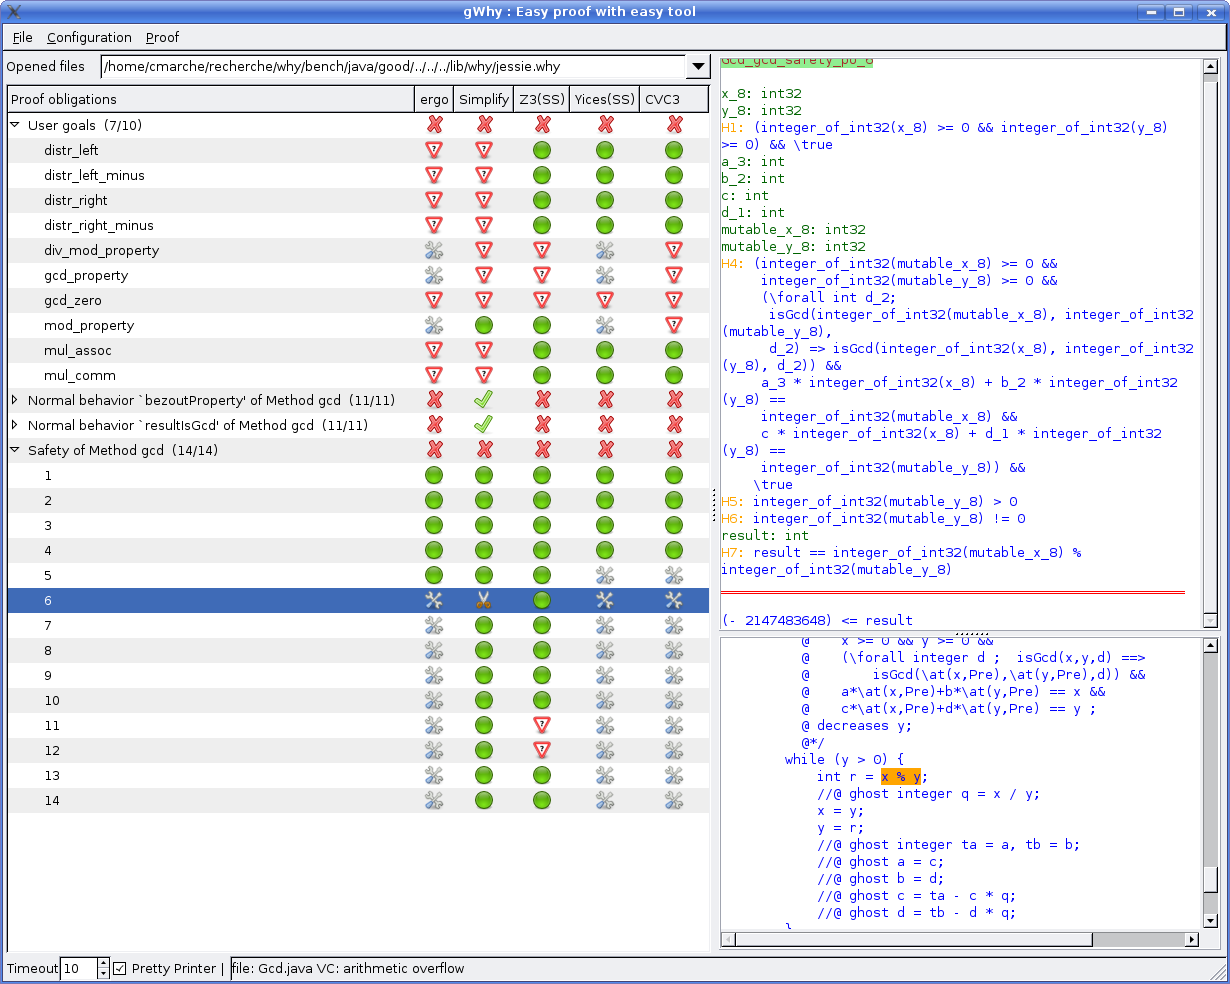
\includegraphics[width=1.08\textwidth]{Gcd1.png}
  \vfill
  \hspace*{-0.04\textwidth}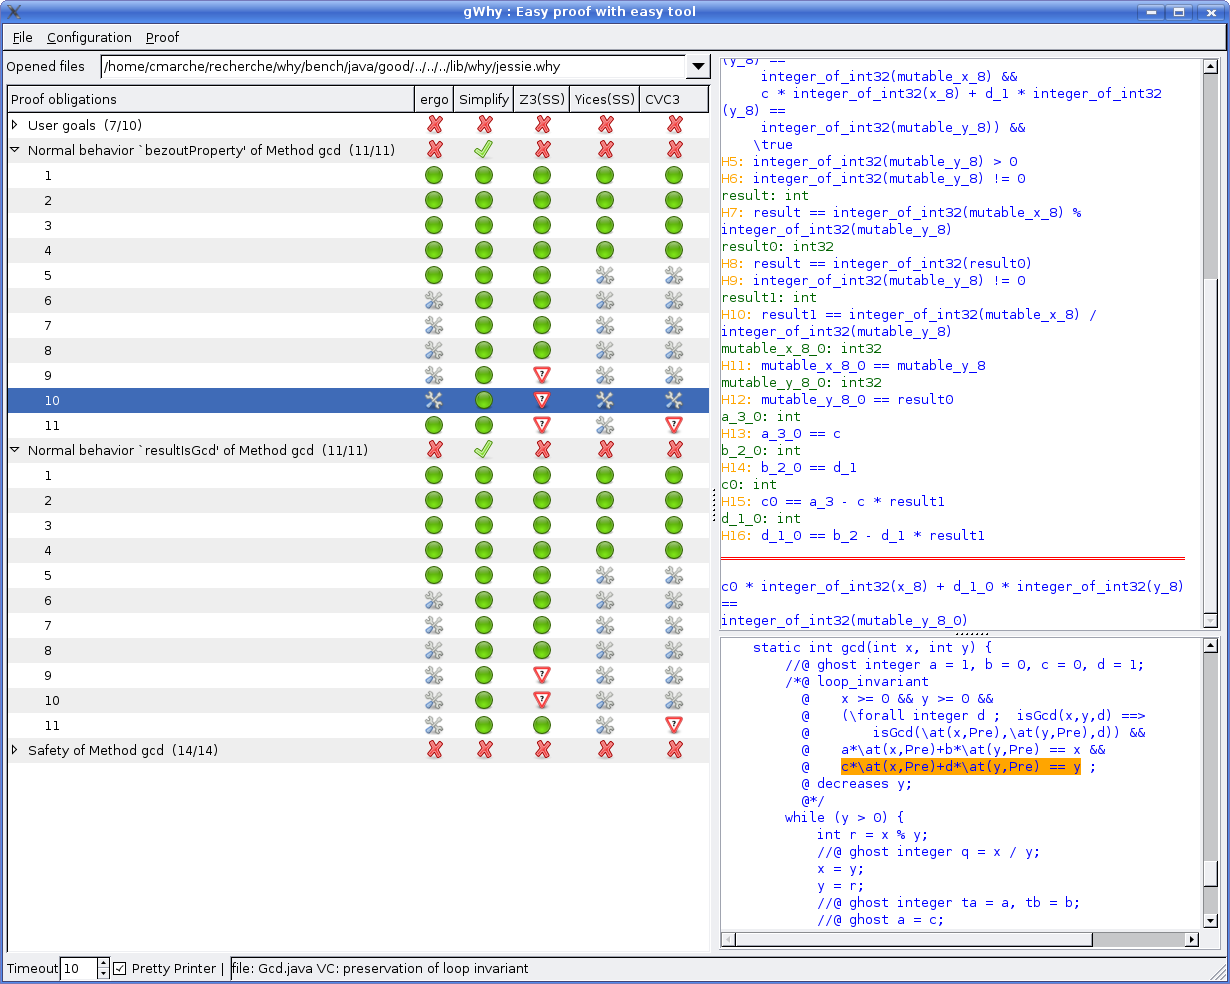
\includegraphics[width=1.08\textwidth]{Gcd2.png}
  \vspace*{-0.07\textheight}
\end{center}


\end{document}

%%% Local Variables: 
%%% mode: latex
%%% TeX-master: t
%%% End: 
